\documentclass[10pt,compress]{beamer}
\usetheme{Madrid}
\usecolortheme{whale}
\usepackage[utf8]{inputenc}
\usepackage[spanish]{babel}
\usepackage{amsmath, amssymb, amsfonts}
\usepackage{graphicx}
\usepackage{booktabs}
\usepackage{multirow}
\usepackage{array}
\usepackage{colortbl}
\usepackage{xcolor}
\decimalpoint

% Configuración de la portada Evaluación de Riesgos por Contaminación Ambiental
\title[Evaluación de Riesgo]{Fundamentos y Metodología de la Evaluación del Riesgo por Tóxicos Atmosféricos}
\subtitle{De la Fuente a la Estimación del Impacto en Salud}
\author[Dr. Agustin García]{Dr. José Agustín García Reynoso}
\institute[ICAyCC]{Instituto de Ciencias de la Atmósfera y Cambio Climático, UNAM}
\logo{
\includegraphics[width=0.8cm] {CCA.png}}

\date{\today}

\begin{document}

\begin{frame}
\titlepage
\end{frame}

% Índice
\begin{frame}{Contenido}
\tableofcontents
\end{frame}

\section{Introducción al Análisis de Riesgo}
\begin{frame}{Introducción}
\begin{itemize}
\item El análisis de riesgos (AR) se desarrolló en los estudios iniciales de juegos de azar en el siglo XVII y con los inicios de la industria aseguradora.
\item Actualmente en la toma de decisiones se emplea el AR en la salud humana y en el ambiente.
\item En esta parte se muestra el proceso de análisis en impactos a la salud.
\end{itemize}
\end{frame}

\section{Terminología}
\begin{frame}{¿Qué es el Riesgo Ambiental?}
    \begin{block}{Definiciones Clave}
        \begin{itemize}
            \item \textbf{Peligro:} Es la fuente del riesgo (la sustancia o agente físico).
            \item \textbf{Riesgo:} Es el \textbf{potencial} de que ocurran consecuencias adversas en la salud o el ambiente debido a la exposición a un peligro.
        \end{itemize}
    \end{block}
    \begin{exampleblock}{Relación}
        El peligro es intrínseco a la sustancia; el riesgo depende de la probabilidad y magnitud de la exposición.
    \end{exampleblock}
\end{frame}

\begin{frame}{Terminología Definiciones}
 \begin{block}{Efectos en la salud}
Son las desviaciones adversas de las funciones normales del organismo.
    \end{block}
 \begin{block}{Exposición}
Concentración pesada en tiempo de un tóxico en las inmediaciones de los puntos de entrada al órgano blanco.
    \end{block}

\begin{itemize}
\item \textbf{Riesgo calculado o estimado}: basado en modelos.
\item \textbf{Riesgo actual}: debido a las condiciones reales.
\item \textbf{Percepción del riesgo}: evaluación individual del riesgo.
\end{itemize}
\end{frame}
%
\begin{frame}{Mediciones del riesgo}
\begin{itemize}
\item Salud humana: casos, incidencia, decesos, pérdida de esperanza de vida.
\item Financiero: dinero (pérdida), ruina.
\item Ecológico: población de especies indicadoras, pérdida de especies, diversidad.
\end{itemize}
\end{frame}

\section{Unidades y Factores}
\begin{frame}{Unidades y factores}
\begin{itemize}
\item Concentración: ppm, ppb, gr/ft$^3$, mg/m$^3$, $\mu$g/m$^3$.
\item Emisión: lb/año, g/s.
\item Factor de dilución: ($\mu$g/m$^3$)/(lb/d).
\item Dosis: mg.
\item Probabilidad de cáncer en el tiempo de vida (LCP).
\item Factor de riesgo unitario por inhalación (URF): LCP/($\mu$g/m$^3$).
\item Factor potencial de ingestión (IPF): LCP/(mg/kg)/d.
\item Factor de Sensibilidad por Edad  \textbf{ASF} ajusta el riesgo por la mayor vulnerabilidad en la infancia.

\end{itemize}
\end{frame}


\begin{frame}{El Factor de Dilución ($\chi/Q$)}
    El factor de dilución, denotado como $(\chi/Q)$, es una herramienta fundamental en la evaluación de riesgos:
    \begin{block}{Definición}
        Es la concentración ambiental modelada ($\chi$) basada en una tasa de emisión unitaria ($Q$) de \textbf{1 gramo por segundo}.
    \end{block}
    \begin{itemize}
        \item Se expresa en unidades de $(\mu g/m^3)/(g/s)$.
        \item Permite calcular rápidamente la concentración de cualquier sustancia multiplicándolo por su tasa de emisión específica: 
        \[ C_{aire} = Q_{sustancia} \times (\chi/Q) \]
    \end{itemize}
\end{frame}

\section{Ejemplos de Análisis de Riesgos}
\begin{frame}{Ejemplo 1: Cálculo de dosis}
Un adulto con rapidez de inhalación de 20 m$^3$/d está sujeto a una concentración de benceno de 2 $\mu$g/m$^3$ durante 48 h.
¿Cuál es la dosis de benceno a los pulmones?
\begin{align*}
D &= \text{Rapidez de inhalación} \times \text{Conc.} \times \text{Tiempo} \\
  &= 20 \, \text{m}^3/\text{d} \times \frac{1 \, \text{d}}{24 \, \text{h}} \times 2 \, \mu\text{g}/\text{m}^3 \times 48 \, \text{h} \\
  &= 80 \, \mu\text{g} \text{ de benceno}
\end{align*}
\end{frame}

\begin{frame}{Ejemplo 2: Cálculo de Riesgo de Cáncer}
    \begin{block}{Problema}
        Una comunidad está expuesta a una concentración promedio de \textbf{Benceno} de $0.5 \mu g/m^3$. Calcule la probabilidad de cáncer en el tiempo de vida (LCP).
    \end{block}
    
    \textbf{Paso 1: Identificar URF.} \\
    Para Benceno, $URF = 2.9 \times 10^{-5} (\mu g/m^3)^{-1}$.
    
    \textbf{Paso 2: Aplicar la fórmula.} \\
    $Riesgo = URF \times Concentraci\acute{o}n$ \\
    $Riesgo = (2.9 \times 10^{-5}) \times 0.5$ \\
    $Riesgo = 1.45 \times 10^{-5}$
    
    \textbf{Resultado:} La probabilidad es de \textbf{14.5 casos por millón} de habitantes.
\end{frame}
\begin{frame}{Ejemplo 3: Índice de Riesgo No Cancerígeno}
    \begin{block}{Problema}
        Se mide una concentración de \textbf{Formaldehído} de $18 \mu g/m^3$ en una zona industrial. Determine si el riesgo es aceptable.
    \end{block}
    
    \textbf{Paso 1: Identificar REL Crónico.} \\
    Para Formaldehído, $REL = 9.0 \mu g/m^3$.
    
    \textbf{Paso 2: Calcular el Índice de Riesgo (IR).} \\
    $IR = \frac{Conc_{medida}}{Conc_{ref}}$ \\
    $IR = \frac{18 \mu g/m^3}{9.0 \mu g/m^3}$ \\
    $IR = 2.0$
    
    \textbf{Interpretación:} Al ser $IR > 1$, existe un riesgo potencial de efectos crónicos adversos y se requieren medidas de control.
\end{frame}

\section{Metodología de Análisis de Riesgo}
\begin{frame}{Metodología}
La metodología sigue cuatro pasos:
\begin{figure}
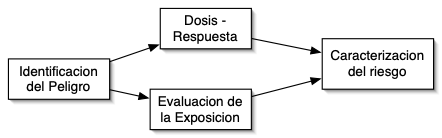
\includegraphics[width=\linewidth]{proceso.png}
\caption{Etapas del análisis de riesgo: identificación de peligros, evaluación de exposición, evaluación de dosis-respuesta, caracterización del riesgo.}
\end{figure}
\end{frame}

\subsection{Identificación}
\begin{frame}{Identificación del peligro}
Determinación e identificación de una sustancia química si es o no causante de un efecto a la salud particular.
\end{frame}
\begin{frame}{Identificación del Peligro: Carcinógenos}
    De acuerdo con las tablas de OEHHA/ARB, identifique los siguientes factores unitarios de riesgo (Inhalation Unit Risk):
    \begin{table}
        \centering
        \begin{tabular}{|l|c|c|}
            \hline
            \textbf{Sustancia} & \textbf{No. CAS} & \textbf{URF $(\mu g/m^3)^{-1}$} \\
            \hline
            Arsénico (Inorgánico) & 7440-38-2 & $3.3 \times 10^{-3}$ \\
            Benceno & 71-43-2 & $2.9 \times 10^{-5}$ \\
            Formaldehído & 50-00-0 & $6.0 \times 10^{-6}$ \\
            Cloruro de Vinilo & 75-01-4 & $7.8 \times 10^{-5}$ \\
            \hline
        \end{tabular}
    \end{table}
    \textit{Nota: Los valores de URF permiten calcular el incremento de probabilidad de contraer cáncer en la vida.}
\end{frame}

\begin{frame}{Recuperación de Valores: No Cancerígenos}
    Identifique los niveles de referencia (REL) para efectos crónicos (inhalación):
    \begin{table}
        \centering
        \begin{tabular}{|l|c|c|}
            \hline
            \textbf{Sustancia} & \textbf{REL Crónico $(\mu g/m^3)$} \\
            \hline
            Acetaldehído & 140 \\
            Acroleína & 0.35 \\
            Benceno & 3.0 \\
            Formaldehído & 9.0 \\
            Mercurio (Inorgánico) & 0.03 \\
            \hline
        \end{tabular}
    \end{table}
    \textit{Si la concentración ambiental supera estos REL, el Índice de Riesgo (IR) será $> 1$, indicando peligro potencial.}
\end{frame}
\begin{frame}{Cálculo de Riesgo de Cáncer}
    El riesgo individual se suma por grupos de edad para reflejar la sensibilidad variable:
    \begin{equation*}
        Riesgo = \sum (Dosis_{edad} \times CPF \times ASF_{edad} \times \frac{ED}{AT})
    \end{equation*}
    \begin{itemize}
        \item \textbf{CPF:} Factor de Potencia Cancerígena ($mg/kg-dia^{-1}$).
        \item \textbf{ED:} Duración de exposición del grupo (años).
        \item \textbf{AT:} Tiempo promedio (30 años para vida residencial)\footnote{ Duración de Exposición: Se ha reducido de 70 a 30 años
para el receptor residencial promedio}.
\item \textbf{ASF:} Se aplica un multiplicador de \textbf{10x} para el tercer trimestre y edades 0-2, y \textbf{3x} para edades 2-16 
    \end{itemize}
   
\end{frame}

\begin{frame}{Efectos No Cancerígenos: Índice de Peligro (HI)}
    Se utiliza el enfoque de umbral mediante los Niveles de Exposición de Referencia (REL) :
    \begin{block}{Cociente de Peligro (HQ)}
        $HQ = \frac{Concentraci\acute{o}n \, Medida}{REL}$ 
    \end{block}
    \begin{itemize}
        \item \textbf{REL:} Concentración segura por debajo de la cual no hay daño.
        \item \textbf{HI:} Suma de los HQ para contaminantes que afectan al mismo órgano blanco.
        \item \textbf{Límite:} Un $HI > 1.0$ indica riesgo potencial.
    \end{itemize}
\end{frame}

\begin{frame}{Aplicación 1: Cálculo de Riesgo de Cáncer}
    \begin{block}{Problema}
        Una comunidad está expuesta a una concentración promedio de \textbf{Benceno} de $0.5 \mu g/m^3$. Calcule la probabilidad de cáncer en el tiempo de vida (LCP).
    \end{block}
    
    \textbf{Paso 1: Identificar URF.} \\
    Para Benceno, $URF = 2.9 \times 10^{-5} (\mu g/m^3)^{-1}$.
    
    \textbf{Paso 2: Aplicar la fórmula.} \\
    $Riesgo = URF \times Concentraci\acute{o}n$ \\
    $Riesgo = (2.9 \times 10^{-5}) \times 0.5$ \\
    $Riesgo = 1.45 \times 10^{-5}$
    
    \textbf{Resultado:} La probabilidad es de \textbf{14.5 casos por millón} de habitantes.
\end{frame}

\begin{frame}{Aplicación 2: Índice de Riesgo No Cancerígeno}
    \begin{block}{Problema}
        Se mide una concentración de \textbf{Formaldehído} de $18 \mu g/m^3$ en una zona industrial. Determine si el riesgo es aceptable.
    \end{block}
    
    \textbf{Paso 1: Identificar REL Crónico.} \\
    Para Formaldehído, $REL = 9.0 \mu g/m^3$.
    
    \textbf{Paso 2: Calcular el Índice de Riesgo (IR).} \\
    $HQ= \frac{Conc_{medida}}{Conc_{ref}}$ \\
    $HQ= \frac{18 \mu g/m^3}{9.0 \mu g/m^3}$ \\
    $HQ= 2.0$
    
    \textbf{Interpretación:} Al ser $HQ> 1$, existe un riesgo potencial de efectos crónicos adversos y se requieren medidas de control.
\end{frame}

\begin{frame}{Aplicación 3: Exposición Multiruta}
    En la evaluación de impacto, el contaminante no solo se inhala.
    \begin{exampleblock}{Caso Práctico}
        Si una empresa emite partículas de Plomo, estas se depositan en el suelo ($C_{suelo}$) y son ingeridas por niños o asimiladas por plantas. 
    \end{exampleblock}
    Para calcular la dosis total ($D$), debemos sumar:
    \begin{center}
        $D_{total} = D_{inhalaci\acute{o}n} + D_{ingesti\acute{o}n} + D_{d\acute{e}rmica}$ 
    \end{center}
    Esto asegura que la protección a la salud considere todas las vías por las que el tóxico entra al organismo.
\end{frame}

\subsection{Evaluación de la Exposición}
\begin{frame}{Evaluación de la Exposición: Rutas y Dosis}
    La exposición ocurre cuando el contaminante entra en contacto con el organismo.
    \begin{itemize}
        \item \textbf{Rutas de Exposición:}
        \begin{itemize}
            \item \textit{Obligatorias:} Inhalación, ingestión de suelo y absorción dérmica.
            \item \textit{Específicas:} Ingestión de agua, alimentos locales o leche materna (para sustancias lipofílicas como dioxinas o plomo).
        \end{itemize}
        \item \textbf{Dosis:} Se calcula en $mg/kg-dia$. Considera la tasa de respiración, peso corporal y tiempo de exposición.
    \end{itemize}
\end{frame}

\begin{frame}{¿Qué es la Exposición?}
    La evaluación de la exposición es el proceso de estimar la magnitud, frecuencia y duración del contacto humano con un agente químico.
    \begin{block}{Definiciones Críticas}
        \begin{itemize}
            \item \textbf{Exposición:} Condición de contacto entre un químico y la frontera de un organismo.
            \item \textbf{Ruta de Exposición:} El camino físico que el químico toma desde la fuente hasta el receptor.
            \item \textbf{Medio Ambiental:} Componentes (aire, suelo, agua) que facilitan la ruta.
        \end{itemize}
    \end{block}
\end{frame}

\section{Clasificación de Sustancias}

\begin{frame}{Inhalación vs. Multiruta}
    \begin{itemize}
        \item \textbf{Sustancias Gaseosas:} La mayoría de los compuestos orgánicos volátiles permanecen en el aire y la \textbf{inhalación} es la ruta de exposición primaria.
        \item \textbf{Sustancias Particuladas:} Los metales y orgánicos semivolátiles se depositan en el suelo, plantas y agua, requiriendo un análisis \textbf{multipathway} (multiruta).
        \item \textbf{Impacto:} El factor multiruta ($MP_c$) se utiliza para considerar todas las rutas adicionales a la inhalación directa.
    \end{itemize}
\end{frame}
\begin{frame}{Flujo del Contaminante en el Ecosistema}
    La siguiente imagen ilustra el transporte de tóxicos atmosféricos hacia el receptor:
    \begin{center}
        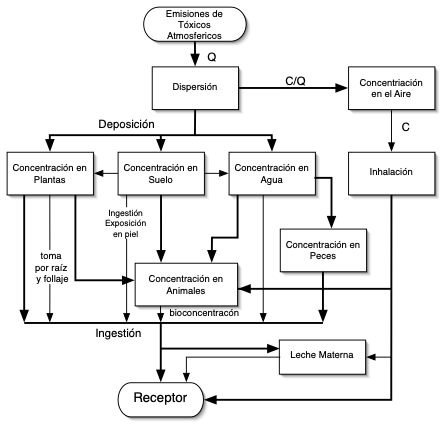
\includegraphics[width=0.5\textwidth]{rutas.png}
    \end{center}
    \small \textbf{Proceso:} Emisión ($Q$) $\rightarrow$ Dispersión $\rightarrow$ Deposición en plantas, suelo y agua $\rightarrow$ Ingestión o Inhalación por el Receptor.
\end{frame}
\begin{frame}{Rutas Obligatorias según el Receptor}
    Para cada escenario de evaluación, se deben incluir rutas mínimas de contacto:
    \begin{table}
        \centering
        \begin{tabular}{|l|c|c|}
            \hline
            \textbf{Ruta de Exposición} & \textbf{Residencial} & \textbf{Trabajador} \\
            \hline
            Inhalación & Obligatoria & Obligatoria \\
            Ingestión de Suelo & Obligatoria & Obligatoria \\
            Exposición Dérmica & Obligatoria & Obligatoria \\
            Consumo de Vegetales & Sitio-específica & No aplica \\
            Leche Materna & Obligatoria* & No aplica \\
            \hline
        \end{tabular}
    \end{table}
    \textit{*Obligatoria si se emiten plomo, dioxinas, furanos, PCBs o PAHs .}
\end{frame}

\begin{frame}{Rutas Sitio-Específicas}
    Dependiendo del entorno de la fuente, se deben evaluar rutas adicionales:
    \begin{itemize}
        \item \textbf{Consumo de Pescado:} Si la instalación impacta cuerpos de agua con pesca local.
        \item \textbf{Productos Animales:} Ingestión de carne, leche de vaca y huevos si hay terrenos de pastoreo o granjas cercanas.
        \item \textbf{Agua Potable:} Si el contaminante se disuelve en reservorios de abasto de agua superficial.
    \end{itemize}
\end{frame}

\begin{frame}{Modelo de Exposición}
\[
E = C \Delta t
\]
donde \(C\) es la concentración promedio y \(\Delta t\) el tiempo de duración.
\[
E_{j,k} = C_{j,k} \Delta t_{j,k}
\]
donde:
\begin{itemize}
\item \(E_{j,k}\): exposición del individuo \(k\) a un contaminante durante \(\Delta t\) en el microambiente \(j\).
\item \(C_{j,k}\): concentración promedio para la persona \(k\) en el microambiente \(j\).
\item \(\Delta t_{j,k}\): tiempo que invierte la persona \(k\) en el microambiente \(j\).
\end{itemize}
\end{frame}

\begin{frame}{Ejemplo de estimación de exposición por ingestión}
Estimar la exposición mediante la ingestión de agua para una persona que trabaja desde los 25 hasta los 65 años en un lugar donde los niveles de HCHO en el agua son de 0.5 $\mu$g/L, consumiendo 1 L/día en el trabajo.
\[
(65-25) \text{ años} \times 250 \text{ días/año} = 10,000 \text{ días}
\]
\[
E = (0.5 \, \mu\text{g/L} \times 1 \, \text{L/día}) \times 10,000 \, \text{días} = 5,000 \, \mu\text{g} = 5 \, \text{mg}
\]
\end{frame}

\begin{frame}{Ejemplo de exposición por inhalación}
Estimar la exposición total a inhalación de HCHO para una persona que trabaja de 25 a 65 años, con niveles de 0.2 $\mu$g/m$^3$ en el trabajo y 0.01 $\mu$g/m$^3$ en la región (fondo). Considere ritmo de inhalación constante de 20 m$^3$/día y 70 años de vida.
\begin{align*}
T_{\text{trabajo}} &= (65-25) \times 250 \times 24 = 240,000 \, \text{h} \\
T_{\text{total}} &= 70 \times 365 \times 24 = 613,200 \, \text{h} \\
T_{\text{no trabajo}} &= 613,200 - 240,000 = 373,200 \, \text{h}
\end{align*}
\[
E = (0.2 \times 240,000 + 0.01 \times 373,200) \, \mu\text{g/m}^3 \cdot \text{h} \times \frac{20 \, \text{m}^3/\text{d}}{24 \, \text{h/d}} = 43,100 \, \mu\text{g} \approx 43 \, \text{mg}
\]
\end{frame}

\begin{frame}{Exposición total}
Estimar la exposición total a formaldehído para un trabajador de 70 kg, usando las exposiciones anteriores y otras fuentes de 1.0 mg.
\[
E_{\text{HCHO}} = E_{\text{aire}} + E_{\text{agua}} + E_{\text{otras fuentes}}
\]
\[
E_{\text{HCHO}} = 43 \, \text{mg} + 5 \, \text{mg} + 1.0 \, \text{mg} = 49 \, \text{mg}
\]
\end{frame}

\begin{frame}{Métodos de evaluación de la exposición}
\begin{itemize}
\item Monitoreo personal (pasivos, activos).
\item Marcadores biológicos (ej. cotinina).
\item Estimados indirectos (modelos).
\end{itemize}
\end{frame}

\begin{frame}{Exposición individual máxima y razonable}
\begin{itemize}
\item \textbf{MEI} (Exposición Individual Máxima): estimado del riesgo asociado con la concentración más alta en un lugar fuera de la industria.
\item \textbf{REI} (Exposición Individual Razonable): estimado del riesgo a una concentración razonable en un lugar fuera de la industria.
\end{itemize}
\[
\text{MEI}_{\text{cron}} = Q_{\text{máx anual}} (\chi/Q), \quad \text{MEI}_{\text{aguda}} = Q_{\text{máx horaria}} (\chi/Q)
\]
\[
\text{REI}_{\text{cron}} = Q_{\text{anual}} (\chi/Q), \quad \text{REI}_{\text{aguda}} = Q_{\text{horaria}} (\chi/Q)
\]
\end{frame}

\begin{frame}{Ejemplo: Exposición a benceno}
Una compañía emite 2 mg/d de benceno. Por mantenimiento, 5 días al año se emite hasta 3 mg/h. El permiso muestra emisión máxima de 4 $\mu$g/s y de 1 g/año. El factor de dilución es 0.01 ($\mu$g/m$^3$)/(g/s) para condiciones crónicas y 1 ($\mu$g/m$^3$)/(g/s) para agudas.
\begin{align*}
\text{MEI}_c &= 1 \, \text{g/año} \times 0.01 \times (3.17\times10^{-8} \, \text{año/s}) = 3.17\times10^{-10} \, \mu\text{g/m}^3 \\
\text{MEI}_a &= 4 \, \mu\text{g/s} \times 1 \times (1 \, \text{g}/10^6 \, \mu\text{g}) = 4\times10^{-6} \, \mu\text{g/m}^3 \\
\text{REI}_c &= 2 \, \text{mg/d} \times 0.01 \times (1 \, \text{g}/10^3 \, \text{mg}) \times (1 \, \text{d}/86,400 \, \text{s}) = 2.3\times10^{-10} \, \mu\text{g/m}^3 \\
\text{REI}_a &= 3 \, \text{mg/h} \times 1 \times (1 \, \text{g}/10^3 \, \text{mg}) \times (1 \, \text{h}/3600 \, \text{s}) = 8.3\times10^{-7} \, \mu\text{g/m}^3
\end{align*}
\end{frame}

\begin{frame}{Ingestión y asimilación}
\begin{itemize}
\item \textbf{Ingestión}: masa de sustancia en contacto con la frontera de intercambio por unidad de peso y tiempo.
\item \textbf{Asimilación}: masa de sustancia absorbida.
\end{itemize}
\[
I_r = C_{\text{aire}} \times \text{Velocidad de inhalación}
\]
\[
I_r = C_{\text{alim}} \times \text{Rapidez de ingestión}
\]
\end{frame}

\begin{frame}{Velocidades de inhalación e ingestión de suelo}
\begin{table}
\centering
\begin{tabular}{lcccc}
\toprule
\textbf{Adulto} & Descanso & Ligero & Moderado & Pesado \\
\midrule
Masc & 0.6 & 1.3 & 2.8 & 7.1 \\
Fem & 0.6 & 1.2 & 4.4 & 4.9 \\
Adulto prom & 0.6 & 1.3 & 2.6 & 6 \\
Niño 10 & 0.4 & 1.7 & 3.3 & 4.2 \\
\bottomrule
\end{tabular}
\caption{Velocidad de inhalación en m$^3$/h. Fuente: U.S. EPA, Superfund Exposure Manual, 1988.}
\end{table}
\begin{table}
\centering
\begin{tabular}{lccccc}
\toprule
\textbf{Meses} & 0-9 & 9-18 & 1.5--3.5 años & 3.5--5 años & 5-18 años \\
\midrule
Ingestión (mg/d) & 0 & 50 & 200 & 50 & 10 \\
\bottomrule
\end{tabular}
\caption{Ingestión de suelo por niños (mg/d). Fuente: U.S. EPA, 1988.}
\end{table}
\end{frame}

\begin{frame}{Asimilación dérmica}
\begin{itemize}
\item La asimilación involucra la absorción de un químico a través de la piel u ojo.
\item Depende del gradiente de concentración, permeabilidad y otros factores.
\end{itemize}
\[
U_r = D_r \times SA_{\text{expuesta}}
\]
\[
D_r = C \times V_d \quad (\text{conc. y velocidad de deposición})
\]
\[
SA = 0.1 \times Peso^{2/3} \, \text{m}^2
\]
\end{frame}

\begin{frame}{Bioconcentración, bioacumulación y biomagnificación}
\begin{itemize}
\item \textbf{Bioconcentración}: incremento en la concentración del tejido vivo sobre la concentración en el medio de exposición.
\item \textbf{Bioacumulación}: proceso de colección de químicos en el tejido vivo.
\item \textbf{Factor de bioconcentración (BCF)}: razón de la concentración en tejido vivo a la del medio de exposición.
\item \textbf{Función de biotransferencia (BTF)}: razón de la concentración en el tejido sobre la ingestión total del químico.
\item \textbf{Biomagnificación}: incremento de la concentración en niveles tróficos superiores.
\end{itemize}
\end{frame}

\begin{frame}{Constantes y factores de bioconcentración}
\begin{table}
\centering
\begin{tabular}{lccc}
\toprule
\textbf{Compuesto} & \(K_{ow}\) & \(\log K_{ow}\) & \(H\) \\
\midrule
Benceno & 1432 & 2.16 & 0.0037 \\
Benzo(a)pireno & 1,097,000 & 6.04 & 0.046 \\
Cloroformo & 87 & 1.94 & 0.0048 \\
Dioxina & 3,900,000 & 6.59 & 2.5 \\
Formaldehído & 1 & 0 & 0.003? \\
Tolueno & 537 & 2.73 & 0.0064 \\
PCB & 7,900,000 & 6.90 & 0.001 \\
\bottomrule
\end{tabular}
\caption{Factores de interceptación (FI) y constantes.}
\end{table}
\end{frame}

\begin{frame}{Factores de bioconcentración suelo-planta, pez, carne}
\begin{table}
\centering
\begin{tabular}{lccc}
\toprule
\textbf{Compuesto} & Suelo-Planta (kg/kg) & Pez (L/kg) & Carne (mg/kg) \\
\midrule
Arsénico & 0.044 & 40 & 0.805 \\
Berilio & 0.011 & 9 & 0.805 \\
Plomo & 0.045 & 49 & 0.0086 \\
Mercurio & 0.93 & 3,000 & 0.01 \\
Níquel & 0.064 & 7 & 0.004 \\
PAH & 0.001-0.33 & 30 & 0.029 \\
Formaldehído & na & na & 2.5E-08 \\
\bottomrule
\end{tabular}
\caption{Factores de bioconcentración.}
\end{table}
\end{frame}

\begin{frame}{Ruta de vegetación}
\begin{itemize}
\item Toma de suelo vía raíces.
\item Deposición directa sobre la planta y toma por hojas.
\item Toma del aire vía el follaje.
\end{itemize}
La concentración total en la planta se determina sumando las concentraciones por cada ruta.
\[
\log \text{BCF} = 1.5888 - 0.578 \log K_{ow}
\]
\[
C_p = \text{BCF} \times C_s
\]
\end{frame}

\begin{frame}{Ruta de vegetación (cont.)}
Por deposición seca y húmeda:
\[
C_p = \frac{C_{\text{aire}} \times V_d \times \text{IF}}{K_{cl} \times \text{CD}}
\]
Por asimilación de gases:
\[
C_p = \frac{C_{\text{aire}} \times R \times T}{H}
\]
\end{frame}

\begin{frame}{Ejemplo: concentración de HCHO en tomates}
Estimar la concentración de HCHO en tomates con exposición a 5 mg/kg en suelo, 0.05 $\mu$g/m$^3$ en aire, velocidad de deposición 0.05 m/s, FI=0.15, eliminación por clima 1.2/día, densidad del cultivo 0.4 kg/m², y \(K_{ow}=1\).
\begin{itemize}
\item Usar las ecuaciones anteriores.
\item Considerar todas las rutas.
\end{itemize}
\end{frame}

\begin{frame}{Ruta de pescado}
Las partículas pueden impactar cuerpos de agua por deposición directa o escorrentía.
\[
C_{\text{pez}} = \text{BCF} \times C_{\text{agua}}
\]
Ejemplo: Mercurio en peces con \(C_{\text{agua}} = 0.02 \, \mu\text{g/m}^3\) y BCF = 33,000 L/kg.
\[
C_{\text{pez}} = 33,000 \times 0.02 \, \mu\text{g/m}^3 \times \frac{1 \, \text{mg}}{1000 \, \mu\text{g}} = 0.66 \, \text{mg/kg}
\]
\end{frame}

\begin{frame}{Ruta de carne}
Ingestión diaria total:
\[
I = I_{ic} + I_{iw} + I_{is} + I_{\text{aire}}
\]
donde:
\begin{itemize}
\item \(I_{ic} = C_{\text{feed}} \times \text{CCR}\) (alimento)
\item \(I_{iw} = C_{\text{agua}} \times \text{WR}\) (agua)
\item \(I_{is} = C_{\text{suelo}} \times \text{SIR}\) (suelo)
\item \(I_{\text{aire}} = C_{\text{aire}} \times \text{IR}\) (inhalación)
\end{itemize}
Concentración en carne:
\[
C_{bm} = I \times \text{BCF} \times \text{FC}
\]
\end{frame}

\subsection{Evaluación de Dosis-Respuesta}
\begin{frame}{Evaluación de Dosis-Respuesta}
Determinación de la relación entre la magnitud de la exposición y la probabilidad de ocurrencia de un efecto a la salud.
\end{frame}
\begin{frame}{Dosis-Respuesta: Carcinógenos vs. No Carcinógenos}
    \begin{columns}
        \column{0.5\textwidth}
        \textbf{Efectos Cancerígenos}:
        \begin{itemize}
            \item Se asume que \textbf{no hay umbral} (cualquier dosis tiene un riesgo).
            \item Se usa el \textbf{CPF} (Factor de Potencia Cancerígena).
        \end{itemize}
        \column{0.5\textwidth}
        \textbf{Efectos No Cancerígenos}:
        \begin{itemize}
            \item Se asume que \textbf{hay un umbral} bajo el cual no hay daño.
            \item Se usa el \textbf{REL} (Nivel de Exposición de Referencia).
        \end{itemize}
    \end{columns}
\end{frame}
\begin{frame}{Ejemplo: Dosis de benzo(a)pireno}
Una empresa incrementa su producción y contaminantes de 1970 a 2020. La concentración de B(a)P en una prisión cercana fue 1.2 $\mu$g/m$^3$ en 1940 y 4.8 $\mu$g/m$^3$ en 2020. ¿Cuál fue la dosis al pulmón de un prisionero durante 50 años?
\begin{eqnarray*}
D &=& 20 \, \text{m}^3/\text{d} \times \frac{(4.8+1.2)}{2} \, \mu\text{g/m}^3 \times 365 \, \text{d/año} \times 50 \, \text{años}\\
& =& 1.1\times10^6 \, \mu\text{g} \\
&=& 1.1 \, \text{g}
\end{eqnarray*}
\end{frame}

\begin{frame}{Definiciones de dosis}
\begin{itemize}
\item \textbf{Efecto a la salud}: desviación adversa de la función normal del cuerpo.
\item \textbf{Agente}: sustancia capaz de producir un efecto.
\item \textbf{Dosis}: cantidad de agente disponible para actuar en el órgano blanco.
\item \textbf{Dosis aplicada}: cantidad presente ante la barrera de absorción.
\item \textbf{Dosis interna}: cantidad que cruzó la barrera de absorción.
\item \textbf{Dosis entregada}: cantidad disponible para interacción con el órgano o célula.
\end{itemize}
\end{frame}

\begin{frame}{Ejemplo: Dosis en ratas}
En un experimento con ratas, el ambiente contiene 3 $\mu$g/m$^3$ de polvo metálico, eficiencia de llegada a pulmones 40\%, y de pulmones a riñones 10\%. Calcule dosis aplicada, interna a pulmones y entregada a riñones para 30 días, con capacidad de inhalación de 0.2 m$^3$/d.
\begin{align*}
D_{\text{aplicada}} &= 0.2 \times 3 \times 30 = 18 \, \mu\text{g} \\
D_{\text{interna}} &= 18 \times 0.40 = 7.2 \, \mu\text{g} \\
D_{\text{entregada}} &= 7.2 \times 0.10 = 0.72 \, \mu\text{g}
\end{align*}
\end{frame}

\begin{frame}{Dosis dependiente de peso y tiempo}
\[
\frac{dD(w)}{dw} = \frac{D}{w}, \quad \frac{dD(t)}{dt} = \frac{D}{t}
\]
Ejemplo: Aspirina 350 mg, 4 tabletas/día para adulto de 70 kg.
\[
\text{Proporción} = \frac{4 \times 350}{70} = 20 \, \text{mg/(kg d)}
\]
\end{frame}

\begin{frame}{Dosis promedio en tiempo de vida}
Ejemplo: Ratones expuestos a arsénico: 6 $\mu$g/d en primer tercio, 12 $\mu$g/d en segundo, 24 $\mu$g/d en tercero.
\[
\text{Dosis promedio} = \frac{1}{3}(6+12+24) = 14 \, \mu\text{g/d}
\]
\end{frame}

\subsection{Caracterización del Riesgo}
\begin{frame}{Caracterización y Estimación del Riesgo}
Descripción de la naturaleza y magnitud del riesgo humano, incluyendo incertidumbre asociada.
    \begin{block}{Riesgo de Cáncer}
        $Riesgo = Dosis \times CPF \times ASF$ \\
        El \textbf{ASF} (Factor de Sensibilidad por Edad) ajusta el riesgo por la mayor vulnerabilidad en la infancia.
    \end{block}
    \begin{block}{Riesgo No Cancerígeno (Hazard Index)}
        $HQ = \frac{Concentraci\acute{o}n}{REL}$ \\
        Si el \textbf{HI} (suma de HQs por órgano blanco) es $> 1.0$, existe un potencial de efectos adversos.
    \end{block}
\end{frame}

\begin{frame}{Índice de Peligro}
A partir de mediciones se puede estimar el HI
\[
\text{HI} = \sum \frac{C_{\text{media}i}}{C_{\text{ref}i}}
\]
\begin{table}
\centering
\begin{tabular}{lccc}
\toprule
\textbf{Contaminante} & Conc. ($\mu$g/m$^3$) & Conc. Ref. ($\mu$g/m$^3$) & HQ \\
\midrule
Ozono & 77.7 & 180 & 0.43 \\
NO$_2$ & 166.9 & 470 & 0.36 \\
SO$_2$ & 46.6 & 66 & 0.07 \\
PM$_{10}$ & 57.9 & 50 & 1.16 \\
HCHO & 10.2 & 3.3 & 3.4 \\\hline
 & & HI =& 5.42\\
\bottomrule
\end{tabular}
\caption{Índice de riesgo para varios contaminantes (Enero-mayo 2002, Merced).}
\end{table}
\end{frame}

\begin{frame}{Riesgo de cáncer}
\[
R = \text{URF} \times \text{Conc.}
\]
donde:
\begin{itemize}
\item \(R\): Probabilidad de Cáncer en el Tiempo de Vida (PCTV).
\item URF: Factor Unitario de Riesgo por inhalación.
\item Conc.: Concentración del compuesto.
\end{itemize}
Pérdida de esperanza de vida:
\[
\text{LLE} = R \times 1.1 \times 10^6 \, \text{días}
\]
\end{frame}

\begin{frame}{Ejemplo: Riesgo ambiental por HCHO}
Para el HCHO ambiental, la PCTV es \(65.3\times10^{-6}\), equivalente a una pérdida de esperanza de vida de 72 días. (Comparar con accidentes de trabajo en EU: 60 días, accidentes en casa: 74 días).
\end{frame}
\begin{frame}{Resumen del Flujo de Evaluación}
    \begin{center}
        \textbf{Emisión (Fuente)} $\rightarrow$ \textbf{Transporte (Dispersión)} $\rightarrow$ \textbf{Dosis (Exposición)} $\rightarrow$ \textbf{Efecto (Dosis-Respuesta)} $\rightarrow$ \textbf{Cálculo de Probabilidad (Riesgo)}.
    \end{center}
    \vspace{1em}
    \textbf{Pregunta de reflexión:} ¿Por qué el riesgo de cáncer se expresa como una probabilidad y el riesgo no cancerígeno como un cociente?.
    \note{ El riesgo cancerígeno se expresa como una probabilidad porque es el resultado de un modelo de extrapolación lineal que no tiene umbral, mientras que el no cancerígeno se expresa como un cociente porque es la relación entre la exposición estimada y un nivel de referencia considerado seguro (que sí tiene umbral)}
\end{frame}
\section{Riesgo a Ecosistemas}
\begin{frame}{Riesgo a Ecosistemas}
Aplicación de técnicas de evaluación de riesgos para mediciones diferentes a la salud humana.
\begin{itemize}
\item Mantenimiento de ecosistemas es importante para la salud humana.
\item Acuerdo de partes interesadas en la medición del riesgo ambiental.
\item Mediciones: especies indicadoras, especies en peligro, comunidades biológicas, diversidad biológica.
\end{itemize}
\end{frame}

\begin{frame}{Ejemplo: Cambios en biodiversidad}
Calcular el cambio en el porcentaje esperado en la diversidad de la comunidad.
\[
\text{BD} = \sum \rho_i \log \rho_i
\]
Datos:
\begin{table}
\centering
\begin{tabular}{lccc}
\toprule
\textbf{Especie} & Población original & Opción A & Opción B \\
\midrule
Hormigas & \(1\times10^6\) & -10\% & -12.5\% \\
Escarabajos & \(1\times10^5\) & -20\% & -12.5\% \\
Aves & \(1\times10^4\) & -25\% & -12.5\% \\
Víboras & \(1\times10^3\) & -50\% & -12.5\% \\
Venado & \(1\times10^2\) & -80\% & -21.5\% \\
\bottomrule
\end{tabular}
\end{table}
\end{frame}

\begin{frame}{Cálculo de biodiversidad}
\[
\text{BD}_{\text{original}} = 10^6(6) + 10^5(5) + 10^4(4) + 10^3(3) + 10^2(2) = 6.54\times10^6
\]
\[
\text{BD}_{\text{opción A}} = 5.78\times10^6, \quad \Delta = 11.6\%
\]
\[
\text{BD}_{\text{opción B}} = 5.67\times10^6, \quad \Delta = 13.4\%
\]
La opción A representa el menor impacto.
\end{frame}

\begin{frame}{AOT40}
AOT40 = suma de las diferencias entre las concentraciones horarias de ozono en la baja atmósfera superiores a 80 $\mu$g/m$^3$ (40 ppb).
\end{frame}

\section{Modelos de Evaluación de Riesgos}
\begin{frame}{Modelos de Evaluación de Riesgos}
\begin{table}
\centering
\begin{tabular}{p{2.5cm}p{3cm}p{4cm}}
\toprule
\textbf{Modelo} & \textbf{Desarrollador} & \textbf{Características} \\
\midrule
HRA 92 & California Air Resources Board & Evaluación multiruta para un contaminante, requiere factores de dilución. \\
ACE2 & California Air Pollution Control Officers Assoc. & Multiruta, multicompuesto, incluye ISCST2 y COMPLEX-I. \\
TOXLT, TOXST & U.S. EPA & Emplean ISCLT2 y ISCST2 para calcular riesgo. \\
HEM-II & U.S. EPA & Acceso automático a archivos de población para riesgo a la población. \\
CalTOX & California Dept. of Toxic Substances Control & Modelo de compartimientos multimedia, incluye modelación probabilística. \\
AERAM & Electric Power Plant Research Institute & Modelo de emisiones de producción eléctrica con combustibles fósiles. \\
TRUE & Electric Power Plant Research Institute & Modelo multitrayectoria. \\
\bottomrule
\end{tabular}
\end{table}
\end{frame}

\section{Comunicación del Riesgo}
\begin{frame}{¿Por qué no basta con la Probabilidad?}
    \begin{itemize}
        \item Expresar el riesgo como ``$10$ chances en un millón'' es útil para reguladores, pero difícil de procesar para el público.
        \item La comunicación efectiva requiere:
        \begin{itemize}
            \item \textbf{Aceptar} al público como un igual.
            \item \textbf{Simplificar} sin perder rigor científico.
            \item \textbf{Contextualizar} el riesgo frente a peligros cotidianos.
        \end{itemize}
    \end{itemize}
\end{frame}
\begin{frame}{Comunicación del Riesgo}
\begin{itemize}
\item Los riesgos son inevitables.
\item Todo cuanto hacemos implica un grado de riesgo.
\item Existen acciones influenciadas por otros (aire contaminado, accidentes).
\item La comunicación del riesgo al público es un reto.
\item La percepción del riesgo es importante en la comunicación.
\end{itemize}
\end{frame}

\begin{frame}{Elementos de la comunicación}
\begin{itemize}
\item \textbf{Mensaje}: información a transmitir.
\item \textbf{Fuente}: punto origen del mensaje.
\item \textbf{Canal}: medio por el cual el mensaje viaja.
\item \textbf{Receptor}: punto final del mensaje.
\end{itemize}
\end{frame}

\begin{frame}{Medios masivos y fuentes oficiales}
\begin{itemize}
\item Los medios masivos consideran un evento noticioso si es sensacionalista o causa alarma.
\item Se da poca información técnica.
\item Los medios buscan respuestas en fuentes oficiales.
\item Las fuentes oficiales usualmente están sesgadas o no tienen autorización de liberar toda la información.
\item Los medios tratan de mostrar dos lados opuestos.
\item Para los reporteros, el peligro es más noticioso que la seguridad.
\end{itemize}
\end{frame}

\begin{frame}{El público}
\begin{itemize}
\item Las políticas públicas tienden a hacer el mayor bien para el mayor número de personas.
\item Esto conduce a la opresión de las minorías.
\item Las reglas de protección son vistas como una amenaza.
\item La gente prefiere tomar decisiones a que las tomen por ellos.
\item Decisiones involuntarias generalmente se sienten injustas y no democráticas.
\end{itemize}
\end{frame}

\begin{frame}{Reglas para comunicar información técnica}
\begin{enumerate}
\item Diga a la gente lo que ha determinado que ellos deben saber.
\item Dígales lo que ellos deben conocer para entender y sentir que entienden la información.
\item Adicione información y guías para preparar a la gente para lo que no se le dice.
\end{enumerate}
\end{frame}

\begin{frame}{Consejos para la comunicación}
\begin{itemize}
\item Acepte e involucre al público como un igual.
\item Planee cuidadosamente y evalúe el desempeño.
\item Escuche a su audiencia.
\item Sea honesto, franco y abierto.
\item Coordine y colabore con otras fuentes creíbles.
\item Satisfaga las necesidades de los medios.
\item Hable claro y con compasión.
\end{itemize}
\end{frame}

\section{Fuente y Dispersión}
\begin{frame}{De la Fuente a la Concentración}
    \begin{itemize}
        \item \textbf{Fuentes:} Pueden ser puntuales (chimeneas), de área (depósitos), de volumen o pozos abiertos.
        \item \textbf{Dispersión Atmosférica:} Modelos como \textbf{AERMOD} o \textbf{CALPUFF} simulan cómo el viento y la topografía transportan los contaminantes.
        \item \textbf{Resultado:} Se obtiene la \textbf{GLC} (Ground Level Concentration), que es la concentración a nivel del suelo donde están los receptores.
    \end{itemize}
\end{frame}

\begin{frame}{¿Qué es una Fuente Puntual?}
    De acuerdo con las guías de la OEHHA y el SCAQMD, las fuentes puntuales son puntos de liberación específicos y confinados, tales como:
    \begin{itemize}
        \item \textbf{Chimeneas de escape} (exhaust stacks).
        \item \textbf{Venteos aislados} de edificios.
    \end{itemize}
    \begin{block}{Parámetros Críticos}
        Para caracterizar una emisión puntual requerimos:
        \begin{enumerate}
            \item Altura y diámetro de la chimenea.
            \item Velocidad de salida del gas ($m/s$).
            \item Temperatura de salida ($K$).
            \item Coordenadas UTM exactas.
        \end{enumerate}
    \end{block}
\end{frame}

\subsection{Método 1: Factores de Emisión}

\begin{frame}{Estimación mediante Factores de Emisión (FE)}
    Este es el método indirecto o teórico. Se basa en la relación entre la cantidad de contaminante generado y el nivel de actividad de la fuente.
    
    \begin{alertblock}{Fórmula Fundamental}
        \[ E = AR \times EF \times (1 - CE) \]
    \end{alertblock}
    
    \textbf{Donde:}
    \begin{itemize}
        \item \textbf{E:} Emisión (ej. $lb/$año o $g/s$).
        \item \textbf{AR (Activity Rate):} Tasa de actividad (ej. galones de combustible quemados).
        \item \textbf{EF (Emission Factor):} Masa de contaminante por unidad de actividad.
        \item \textbf{CE (Control Efficiency):} Eficiencia del equipo de control (filtros, lavadores).
    \end{itemize}
\end{frame}

\subsection{Método 2: Mediciones en Chimenea}

\begin{frame}{Mediciones Directas (Source Tests)}
    Las mediciones en chimenea representan el escenario más real y deben realizarse bajo protocolos aprobados (como los del South Coast AQMD).
    
    \begin{block}{Cálculo de la Tasa de Emisión ($Q$)}
        La emisión se determina multiplicando la concentración medida del contaminante por el flujo volumétrico del gas.
        \[ Q = C_{medida} \times V_{flow} \]
    \end{block}
    
    \begin{itemize}
        \item \textbf{$C_{medida}$:} Concentración del contaminante (ej. $mg/m^3$).
        \item \textbf{$V_{flow}$:} Flujo de gas en la chimenea (ACFM o $m^3/s$).
    \end{itemize}
\end{frame}

\subsection{Comparativa y Reporte}

\begin{frame}{Unidades de Reporte y Frecuencia}
    Para una Evaluación de Riesgo a la Salud (ERS), las emisiones deben cuantificarse en dos escalas temporales:
    
    \begin{enumerate}
        \item \textbf{Promedio Anual ($lb/yr$ o $g/s$):} Se utiliza para evaluar riesgos de \textbf{cáncer} y efectos \textbf{crónicos} no cancerígenos.
        \item \textbf{Máxima Horaria ($lb/hr$ o $g/s$):} Es crítica para evaluar efectos \textbf{agudos} (exposiciones de corto plazo).
    \end{enumerate}
    
    \textit{Nota: Los reportes deben indicar claramente si los valores fueron medidos o estimados.}
\end{frame}

\subsection{Ejemplo de Aplicación}

\begin{frame}{Ejemplo Práctico}
    \begin{exampleblock}{Caso}
        Una caldera quema 10,000 galones de Diesel al año. El factor de emisión para partículas es de 2 $lb/1000$ gal. ¿Cuál es su emisión anual?
    \end{exampleblock}
    
    \textbf{Resolución:}
    \begin{itemize}
        \item $AR = 10,000$ gal/año
        \item $EF = 0.002$ lb/gal
        \item $E = 10,000 \times 0.002 = \textbf{20 lb/año}$
    \end{itemize}
    \vspace{1em}
    \textbf{Pregunta de reflexión:} Si instalamos un ciclón con 90\% de eficiencia ($CE=0.90$), ¿cuántas libras se liberarían realmente a la atmósfera?.
\end{frame}

\subsection{Conceptos Clave de dispersión}

\begin{frame}{Altura Física vs. Altura Efectiva ($H$)}
    En el modelado de fuentes puntuales, el contaminante no sale simplemente de la chimenea, sino que asciende debido a su impulso y temperatura:
    \begin{itemize}
        \item \textbf{Altura Física ($h_s$):} La altura estructural de la chimenea (en este caso, 20 m).
        \item \textbf{Altura Efectiva ($H$):} La altura real desde donde comienza la dispersión horizontal tras el ascenso de la pluma (en este caso, 60 m).
    \end{itemize}
    \begin{exampleblock}{Dato Crítico}
        El modelo gaussiano utiliza la \textbf{altura efectiva ($H=60m$)} para calcular el impacto a nivel del suelo.
    \end{exampleblock}
\end{frame}
\begin{frame}{Factor de Dilución ($\chi$/Q)}
\begin{itemize}
\item Valores de $\chi$/Q en unidades de [($\mu$g/m$^3$)/(lb/d)]
\item Escenario de operación: 24 horas al día, 365 días al año
\end{itemize}
\vspace{0.3cm}
\begin{table}[h]
\centering
\small
\setlength{\tabcolsep}{3pt}
\begin{tabular}{c|cccccccc}
\toprule
\multirow{2}{*}{\textbf{Altura de}} & \multicolumn{8}{c}{\textbf{Distancia a la barda (m)}} \\
\cline{2-9}
\textbf{Chimenea (ft)} & 10-25 & 25-50 & 50-75 & 75-100 & 100-150 & 150-200 & 200-250 & 250-300 \\
\midrule
13-25 & 24.45 & 14.16 & 6.44 & 3.63 & 2.33 & 1.20 & 0.73 & 0.50 \\
25-50 & 3.57 & 3.31 & 2.47 & 2.47 & 1.81 & 1.05 & 0.67 & 0.47 \\
$>$50 & 0.52 & 0.52 & 0.52 & 0.52 & 0.48 & 0.48 & 0.41 & 0.33 \\
\bottomrule
\end{tabular}
\caption{Factores de dilución $\chi$/Q [($\mu$g/m$^3$)/(lb/d)] para diferentes alturas de chimenea y distancias a la barda.}
\label{tab:dilucion}
\end{table}
\end{frame}
%\section{Modelo Gaussiano}

\begin{frame}{La Ecuación de Dispersión Gaussiana}
    Para receptores a nivel del suelo ($z=0$) y en la línea central del viento ($y=0$), la ecuación es:
    \begin{equation*}
        \chi(x) = \frac{Q}{\pi \sigma_y \sigma_z u} \exp\left( -\frac{1}{2} \frac{H^2}{\sigma_z^2} \right)
    \end{equation*}
    \textbf{Variables involucradas:}
    \begin{itemize}
        \item \textbf{$x$:} Distancia a la fuente (500 m).
        \item \textbf{$\sigma_y, \sigma_z$:} Coeficientes de dispersión (dependen de la estabilidad D).
        \item \textbf{$u$:} Velocidad del viento.
        \item \textbf{$H$:} Altura efectiva (60 m) [2].
    \end{itemize}
\end{frame}

%\section{Aplicación Práctica}


\section{Ejercicios}
\begin{frame}{Ejercicio 1: Cálculo de dosis}
Un adulto con rapidez de inhalación de 15 m$^3$/d está expuesto a una concentración de tolueno de 5 $\mu$g/m$^3$ durante 72 horas. Calcule la dosis de tolueno en los pulmones.
\end{frame}

\begin{frame}{Ejercicio 2: Riesgo por arsénico}
Calcule la PCTV para una exposición crónica de 0.5 ng/m$^3$ de arsénico, si el URF = 1.4×10$^{-3}$.
\end{frame}

\begin{frame}{Ejercicio 3: Exposición por ingestión}
Una persona consume 2 L/día de agua con 0.2 $\mu$g/L de benceno durante 30 años. Calcule la exposición total.
\end{frame}

\begin{frame}{Ejercicio 4: Índice de riesgo}
Calcule el IR para una concentración de PM$_{2.5}$ de 25 $\mu$g/m$^3$ si la concentración de referencia es 12 $\mu$g/m$^3$.
\end{frame}

\begin{frame}{Ejercicio 5: Biodiversidad}
Con los datos del ejemplo de biodiversidad, calcule el cambio porcentual en BD si la población de hormigas se reduce en un 20\%, escarabajos en 15\%, aves en 10\%, víboras en 5\% y venados en 2\%.
\end{frame}
\begin{frame}{Ejercicio 6: Estabilidad D y Distancia de 500 m}
    \begin{itemize}
        \item \textbf{Estabilidad D:} Representa condiciones neutras (frecuentes en días nublados o con viento moderado).
        \item \textbf{A 500 metros:} Los coeficientes $\sigma_y$ (dispersión horizontal) y $\sigma_z$ (dispersión vertical) se obtienen de tablas o curvas de Pasquill-Gifford.
    \end{itemize}
    \begin{block}{Interpretación}
        Una mayor estabilidad vertical (como la clase F) resultaría en una pluma más estrecha y concentraciones más altas, mientras que la \textbf{estabilidad D} permite una dilución moderada antes de tocar el suelo.
    \end{block}
\end{frame}
\section{Ejercicio 7: Aplicación Práctica}

\begin{frame}{Cálculo de la Concentración a 400 metros}
    \begin{block}{Parámetros del Escenario}
        \begin{itemize}
            \item \textbf{Distancia ($x$):} 400 m.
            \item \textbf{Altura Efectiva ($H$):} 60 m.
            \item \textbf{Estabilidad D:} $\sigma_y = 29\text{ m}$, $\sigma_z = 15\text{ m}$.
            \item \textbf{Velocidad del viento ($u$):} Se asume $1\text{ m/s}$ para cálculo unitario.
        \end{itemize}
    \end{block}

    \textbf{Paso 1: Evaluar el término exponencial (Efecto de la altura):}
    \[ \exp\left( -0.5 \cdot \frac{H^2}{\sigma_z^2} \right) = \exp\left( -0.5 \cdot \frac{60^2}{15^2} \right) = \exp(-8) \approx 0.000335 \]

    \textbf{Paso 2: Calcular el factor de dilución ($\chi/Q$):}
    \[ \frac{\chi}{Q} = \frac{1}{\pi \cdot 29 \cdot 15 \cdot 1} \cdot 0.000335 \approx 2.45 \times 10^{-7} \frac{\mu g/m^3}{g/s} \]

    \textit{Nota: Este valor representa la capacidad de la atmósfera para diluir el contaminante en este punto específico.}
\end{frame}

\begin{frame}{Análisis de Comprensión}
    \begin{alertblock}{Comparación con el caso anterior}
        Al reducir la distancia de 500 m a 400 m, los valores de $\sigma$ disminuyen. ¿Cómo afecta esto a la dosis recibida por el receptor?
    \end{alertblock}
    \begin{itemize}
        \item \textbf{Relación causa-efecto:} Valores de $\sigma$ más pequeños implican una pluma menos dispersa (más concentrada).
        \item \textbf{Impacto de la altura:} Dado que $H=60m$ y $\sigma_z=15m$, el receptor está "lejos" del núcleo de la pluma ($H > 2\sigma_z$), lo que resulta en una concentración a nivel del suelo muy baja en este punto.
        \item \textbf{Conclusión didáctica:} La dispersión no solo depende de la distancia, sino de la relación entre la altura de emisión y la capacidad de mezcla vertical.
    \end{itemize}
\end{frame}

\section{Referencias}
\begin{frame}{Referencias}
\begin{thebibliography}{9}
\bibitem{epa1988} U.S. Environmental Protection Agency. (1988). \emph{Superfund Exposure Manual}. EPA/540/1-88/001. Office of Remedial Response, Washington, DC.
\bibitem{oehha2024} Office of Environmental Health Hazard Assessment (OEHHA) and California Air Resources Board (ARB). (2024). \emph{Consolidated Table of OEHHA/ARB Approved Risk Assessment Health Values}. Table last updated: December 17, 2024.
\bibitem{oehha2009} OEHHA. (2009). \emph{Air Toxics Hot Spots Program Technical Support Document for Cancer Potencies}. Sacramento, CA.
\bibitem{oehha2012} OEHHA. (2012). \emph{Air Toxics Hot Spots Program Technical Support Document for Exposure Assessment and Stochastic Analysis}. Sacramento, CA.
\bibitem{oehha2015} OEHHA. (2015). \emph{Guidance Manual for the Preparation of Risk Assessments}. Sacramento, CA.
\bibitem{grutter2002} Grutter, M. (2002). Datos de la Red Automática de Monitoreo Ambiental (RAMA), enero-mayo 2002, Merced.
\bibitem{grat1996} Gratt, L.B. (1996). \emph{Air Toxic Risk Assessment and Management}. Van Nostrand Reinhold.
\end{thebibliography}
\end{frame}

\begin{frame}{Aplicación del Factor de Dilución ($\chi$/Q)}
\begin{block}{Contexto importante}
\begin{itemize}
\item La tabla de $\chi$/Q se aplica para \textbf{exposición pasiva} en la \textbf{barda perimetral} de una instalación.
\item Los valores son típicos para \textbf{condiciones de estabilidad atmosférica promedio} (clase D de Pasquill-Gifford).
\item Para condiciones de \textbf{inversión térmica extrema}, se requieren factores más conservadores (peor escenario).
\item El factor de dilución convierte la \textbf{emisión (Q)} en \textbf{concentración en aire ($\chi$)} en el punto de interés.
\end{itemize}
\end{block}
\end{frame}

\begin{frame}{Ejemplo de Cálculo con Factor de Dilución}
\begin{exampleblock}{Problema}
Una empresa emite \textbf{2.5 lb/día} de benceno desde una chimenea de \textbf{30 ft} de altura. 
La barda perimetral de la instalación se encuentra a \textbf{60 m} de distancia.

Calcule la concentración de benceno en el aire en la barda.
\end{exampleblock}
\vspace{0.3cm}

\pause

\begin{block}{Solución}
\begin{enumerate}
\item Identificar el factor de dilución de la tabla:
\begin{itemize}
\item Altura: 25-50 ft → fila 2
\item Distancia: 50-75 m → columna 3
\item $\chi$/Q = \textbf{2.47} ($\mu$g/m$^3$)/(lb/d)
\end{itemize}
\item Aplicar la fórmula:
\[
C_{\text{aire}} = Q \times (\chi/Q)
\]
\[
C_{\text{aire}} = 2.5 \, \text{lb/d} \times 2.47 \, \frac{\mu\text{g/m}^3}{\text{lb/d}} = \textbf{6.175} \, \mu\text{g/m}^3
\]
\end{enumerate}
\end{block}
\end{frame}

\begin{frame}{Interpretación del Resultado}
\begin{itemize}
\item La concentración estimada en la barda es de \textbf{6.175 $\mu$g/m$^3$} de benceno.
\item \textbf{Comparación}: El valor de referencia crónico (REL) para benceno es 3.0 $\mu$g/m$^3$ (OEHHA, 2014).
\item \textbf{Índice de Riesgo (no cancerígeno)}:
\[
\text{IR} = \frac{C_{\text{aire}}}{\text{REL}} = \frac{6.175}{3.0} = 2.06
\]
\textcolor{red}{IR $>$ 1} → La exposición supera el nivel de referencia.
\item \textbf{Riesgo cancerígeno} (URF benceno = 2.9×$^{-8}$):
\[
\text{PCTV} = \text{URF} \times C_{\text{aire}} = 2.9\times10^{-5} \times 6.175 = 1.79\times10^{-4}
\]
Equivale a \textbf{179 casos por millón} (o $1.79 \times 10^{-4}$).
\end{itemize}
\vspace{0.2cm}
\begin{alertblock}{Nota}
Este es un ejemplo ilustrativo. En la práctica, se deben considerar todas las rutas de exposición (inhalación, ingestión, dérmica) y múltiples contaminantes.
\end{alertblock}
\end{frame}

\begin{frame}{Sensibilidad del Factor de Dilución}
\begin{itemize}
\item \textbf{¿Qué pasa si la chimenea fuera más alta?}
\begin{itemize}
\item Altura >50 ft, misma distancia (50-75 m): $\chi$/Q = 0.52
\item \(C_{\text{aire}} = 2.5 \times 0.52 = 1.30 \, \mu\text{g/m}^3\) (¡5 veces menor!)
\end{itemize}
\item \textbf{¿Y si la barda estuviera más cerca?}
\begin{itemize}
\item Misma altura (25-50 ft), distancia 10-25 m: $\chi$/Q = 3.57
\item \(C_{\text{aire}} = 2.5 \times 3.57 = 8.925 \, \mu\text{g/m}^3\) (45\% mayor)
\end{itemize}
\end{itemize}
\vspace{0.3cm}
\begin{center}
\color{blue}
\textbf{Conclusión:} La altura de la chimenea y la distancia al receptor \textbf{impactan significativamente} la concentración estimada.
\end{center}
\end{frame}
\end{document}
